\documentclass[]{article}
\usepackage{lmodern}
\usepackage{amssymb,amsmath}
\usepackage{ifxetex,ifluatex}
\usepackage{fixltx2e} % provides \textsubscript
\ifnum 0\ifxetex 1\fi\ifluatex 1\fi=0 % if pdftex
  \usepackage[T1]{fontenc}
  \usepackage[utf8]{inputenc}
\else % if luatex or xelatex
  \ifxetex
    \usepackage{mathspec}
  \else
    \usepackage{fontspec}
  \fi
  \defaultfontfeatures{Ligatures=TeX,Scale=MatchLowercase}
\fi
% use upquote if available, for straight quotes in verbatim environments
\IfFileExists{upquote.sty}{\usepackage{upquote}}{}
% use microtype if available
\IfFileExists{microtype.sty}{%
\usepackage{microtype}
\UseMicrotypeSet[protrusion]{basicmath} % disable protrusion for tt fonts
}{}
\usepackage[margin=1in]{geometry}
\usepackage{hyperref}
\hypersetup{unicode=true,
            pdftitle={Homework 4 - Key},
            pdfborder={0 0 0},
            breaklinks=true}
\urlstyle{same}  % don't use monospace font for urls
\usepackage{color}
\usepackage{fancyvrb}
\newcommand{\VerbBar}{|}
\newcommand{\VERB}{\Verb[commandchars=\\\{\}]}
\DefineVerbatimEnvironment{Highlighting}{Verbatim}{commandchars=\\\{\}}
% Add ',fontsize=\small' for more characters per line
\usepackage{framed}
\definecolor{shadecolor}{RGB}{248,248,248}
\newenvironment{Shaded}{\begin{snugshade}}{\end{snugshade}}
\newcommand{\KeywordTok}[1]{\textcolor[rgb]{0.13,0.29,0.53}{\textbf{#1}}}
\newcommand{\DataTypeTok}[1]{\textcolor[rgb]{0.13,0.29,0.53}{#1}}
\newcommand{\DecValTok}[1]{\textcolor[rgb]{0.00,0.00,0.81}{#1}}
\newcommand{\BaseNTok}[1]{\textcolor[rgb]{0.00,0.00,0.81}{#1}}
\newcommand{\FloatTok}[1]{\textcolor[rgb]{0.00,0.00,0.81}{#1}}
\newcommand{\ConstantTok}[1]{\textcolor[rgb]{0.00,0.00,0.00}{#1}}
\newcommand{\CharTok}[1]{\textcolor[rgb]{0.31,0.60,0.02}{#1}}
\newcommand{\SpecialCharTok}[1]{\textcolor[rgb]{0.00,0.00,0.00}{#1}}
\newcommand{\StringTok}[1]{\textcolor[rgb]{0.31,0.60,0.02}{#1}}
\newcommand{\VerbatimStringTok}[1]{\textcolor[rgb]{0.31,0.60,0.02}{#1}}
\newcommand{\SpecialStringTok}[1]{\textcolor[rgb]{0.31,0.60,0.02}{#1}}
\newcommand{\ImportTok}[1]{#1}
\newcommand{\CommentTok}[1]{\textcolor[rgb]{0.56,0.35,0.01}{\textit{#1}}}
\newcommand{\DocumentationTok}[1]{\textcolor[rgb]{0.56,0.35,0.01}{\textbf{\textit{#1}}}}
\newcommand{\AnnotationTok}[1]{\textcolor[rgb]{0.56,0.35,0.01}{\textbf{\textit{#1}}}}
\newcommand{\CommentVarTok}[1]{\textcolor[rgb]{0.56,0.35,0.01}{\textbf{\textit{#1}}}}
\newcommand{\OtherTok}[1]{\textcolor[rgb]{0.56,0.35,0.01}{#1}}
\newcommand{\FunctionTok}[1]{\textcolor[rgb]{0.00,0.00,0.00}{#1}}
\newcommand{\VariableTok}[1]{\textcolor[rgb]{0.00,0.00,0.00}{#1}}
\newcommand{\ControlFlowTok}[1]{\textcolor[rgb]{0.13,0.29,0.53}{\textbf{#1}}}
\newcommand{\OperatorTok}[1]{\textcolor[rgb]{0.81,0.36,0.00}{\textbf{#1}}}
\newcommand{\BuiltInTok}[1]{#1}
\newcommand{\ExtensionTok}[1]{#1}
\newcommand{\PreprocessorTok}[1]{\textcolor[rgb]{0.56,0.35,0.01}{\textit{#1}}}
\newcommand{\AttributeTok}[1]{\textcolor[rgb]{0.77,0.63,0.00}{#1}}
\newcommand{\RegionMarkerTok}[1]{#1}
\newcommand{\InformationTok}[1]{\textcolor[rgb]{0.56,0.35,0.01}{\textbf{\textit{#1}}}}
\newcommand{\WarningTok}[1]{\textcolor[rgb]{0.56,0.35,0.01}{\textbf{\textit{#1}}}}
\newcommand{\AlertTok}[1]{\textcolor[rgb]{0.94,0.16,0.16}{#1}}
\newcommand{\ErrorTok}[1]{\textcolor[rgb]{0.64,0.00,0.00}{\textbf{#1}}}
\newcommand{\NormalTok}[1]{#1}
\usepackage{longtable,booktabs}
\usepackage{graphicx,grffile}
\makeatletter
\def\maxwidth{\ifdim\Gin@nat@width>\linewidth\linewidth\else\Gin@nat@width\fi}
\def\maxheight{\ifdim\Gin@nat@height>\textheight\textheight\else\Gin@nat@height\fi}
\makeatother
% Scale images if necessary, so that they will not overflow the page
% margins by default, and it is still possible to overwrite the defaults
% using explicit options in \includegraphics[width, height, ...]{}
\setkeys{Gin}{width=\maxwidth,height=\maxheight,keepaspectratio}
\IfFileExists{parskip.sty}{%
\usepackage{parskip}
}{% else
\setlength{\parindent}{0pt}
\setlength{\parskip}{6pt plus 2pt minus 1pt}
}
\setlength{\emergencystretch}{3em}  % prevent overfull lines
\providecommand{\tightlist}{%
  \setlength{\itemsep}{0pt}\setlength{\parskip}{0pt}}
\setcounter{secnumdepth}{0}
% Redefines (sub)paragraphs to behave more like sections
\ifx\paragraph\undefined\else
\let\oldparagraph\paragraph
\renewcommand{\paragraph}[1]{\oldparagraph{#1}\mbox{}}
\fi
\ifx\subparagraph\undefined\else
\let\oldsubparagraph\subparagraph
\renewcommand{\subparagraph}[1]{\oldsubparagraph{#1}\mbox{}}
\fi

%%% Use protect on footnotes to avoid problems with footnotes in titles
\let\rmarkdownfootnote\footnote%
\def\footnote{\protect\rmarkdownfootnote}

%%% Change title format to be more compact
\usepackage{titling}

% Create subtitle command for use in maketitle
\newcommand{\subtitle}[1]{
  \posttitle{
    \begin{center}\large#1\end{center}
    }
}

\setlength{\droptitle}{-2em}

  \title{Homework 4 - Key}
    \pretitle{\vspace{\droptitle}\centering\huge}
  \posttitle{\par}
  \subtitle{Math 530/630}
  \author{}
    \preauthor{}\postauthor{}
    \date{}
    \predate{}\postdate{}
  

\begin{document}
\maketitle

\begin{enumerate}
\def\labelenumi{\arabic{enumi}.}
\item
  One of the goals of the Edinburgh Artery Study was to investigate the
  risk factors for peripheral arterial disease among persons 55 to 75
  years of age.You wish to compare mean LDL cholesterol levels, measured
  in mmol/liter, among four different populations of subjects: patients
  with intermittent claudication or interruptions in movement, those
  with major asymptomatic disease, those with minor asymptomatic
  disease, and those with no evidence of disease at all. Samples are
  selected from each population; summary statistics are shown below:

  \begin{enumerate}
  \def\labelenumii{\alph{enumii}.}
  \tightlist
  \item
    Use a one-way ANOVA to test the null hypothesis that the mean LDL
    cholesterol levels are the same for each of the four populations.
    Calculate this by-hand, and include your ANOVA table.\\
  \item
    If \(\alpha=.05\), what do you conclude?
  \item
    What assumptions about the data must be true for you to use one-way
    ANOVA?
  \item
    Is it necessary to take any additional steps in this analysis? If
    so, what?
  \end{enumerate}
\end{enumerate}

\begin{longtable}[]{@{}llll@{}}
\toprule
& \(n\) & \(\bar{x}\) & \(s\)\tabularnewline
\midrule
\endhead
Intermittent Claudation & 73 & 6.22 & 1.62\tabularnewline
Major Asymptomatic Disease & 105 & 5.81 & 1.43\tabularnewline
Minor Asymptomatic Disease & 240 & 5.77 & 1.24\tabularnewline
No Disease & 1080 & 5.47 & 1.31\tabularnewline
\bottomrule
\end{longtable}

Answers

\begin{enumerate}
\def\labelenumi{\alph{enumi}.}
\item
\end{enumerate}

\begin{Shaded}
\begin{Highlighting}[]
\NormalTok{ns =}\StringTok{ }\KeywordTok{c}\NormalTok{(}\DecValTok{73}\NormalTok{, }\DecValTok{105}\NormalTok{, }\DecValTok{240}\NormalTok{, }\DecValTok{1080}\NormalTok{)}
\NormalTok{means =}\StringTok{ }\KeywordTok{c}\NormalTok{(}\FloatTok{6.22}\NormalTok{, }\FloatTok{5.81}\NormalTok{, }\FloatTok{5.77}\NormalTok{, }\FloatTok{5.47}\NormalTok{)}
\NormalTok{grand_mean =}\StringTok{ }\KeywordTok{mean}\NormalTok{(means)}
\NormalTok{sigmas =}\StringTok{ }\KeywordTok{c}\NormalTok{(}\FloatTok{1.62}\NormalTok{, }\FloatTok{1.43}\NormalTok{, }\FloatTok{1.24}\NormalTok{, }\FloatTok{1.31}\NormalTok{)}
\NormalTok{ttl_n =}\StringTok{ }\KeywordTok{sum}\NormalTok{(ns)}
\NormalTok{df_between_groups =}\StringTok{ }\KeywordTok{length}\NormalTok{(ns) }\OperatorTok{-}\StringTok{ }\DecValTok{1} 
\NormalTok{df_within_groups =}\StringTok{ }\NormalTok{ttl_n }\OperatorTok{-}\StringTok{ }\DecValTok{1}
\NormalTok{SSW_var =}\StringTok{ }\KeywordTok{sum}\NormalTok{((ns}\OperatorTok{-}\DecValTok{1}\NormalTok{)}\OperatorTok{*}\NormalTok{sigmas}\OperatorTok{^}\DecValTok{2}\NormalTok{)}\OperatorTok{/}\NormalTok{df_within_groups}
\NormalTok{x_bar =}\StringTok{ }\KeywordTok{sum}\NormalTok{(ns}\OperatorTok{*}\NormalTok{means)}\OperatorTok{/}\NormalTok{ttl_n}
\NormalTok{SSB_var =}\StringTok{ }\KeywordTok{sum}\NormalTok{(ns}\OperatorTok{*}\NormalTok{(means}\OperatorTok{-}\NormalTok{x_bar)}\OperatorTok{^}\DecValTok{2}\NormalTok{)}\OperatorTok{/}\NormalTok{df_between_groups}
\NormalTok{(}\DataTypeTok{F_stat =}\NormalTok{ SSB_var}\OperatorTok{/}\NormalTok{SSW_var)}
\end{Highlighting}
\end{Shaded}

\begin{verbatim}
## [1] 10.88783
\end{verbatim}

\begin{Shaded}
\begin{Highlighting}[]
\NormalTok{(}\DataTypeTok{F_crit =} \KeywordTok{qf}\NormalTok{(.}\DecValTok{95}\NormalTok{,}\DecValTok{3}\NormalTok{,}\DecValTok{1494}\NormalTok{))}
\end{Highlighting}
\end{Shaded}

\begin{verbatim}
## [1] 2.610859
\end{verbatim}

\begin{enumerate}
\def\labelenumi{\alph{enumi}.}
\setcounter{enumi}{1}
\item
\end{enumerate}

\begin{itemize}
\tightlist
\item
  F(3,1494) = 10.87
\item
  F\_crit = 2.61
\item
  F(3,1494) = 10.87 \textgreater{} F\_crit=2.61
\item
  We can reject the null hypothesis, that LDL Cholesterol is the same
  for all the four groups.
\end{itemize}

\begin{enumerate}
\def\labelenumi{\alph{enumi}.}
\setcounter{enumi}{2}
\tightlist
\item
  Assumptions for one way ANOVA:
\end{enumerate}

\begin{itemize}
\tightlist
\item
  The k samples are randomly selected from the k populations of interest
\item
  Each of the k populations have a normal distribution
\item
  All k populations have the same variance
\end{itemize}

\begin{enumerate}
\def\labelenumi{\alph{enumi}.}
\setcounter{enumi}{3}
\tightlist
\item
  The ANOVA F-test answers the question whether there are significant
  differences in the 4 population means. However, it does not provide us
  with any information about how they differ. Therefore when we reject
  H0 in ANOVA, additional analyses are required to determine what is
  driving the difference in means. The function pairwise.t.test computes
  the pair-wise comparisons between group means with corrections for
  multiple testing.
\end{enumerate}

pairwise.t.test(reponse, factor, p.adjust = method, alternative =
c(``two.sided'', ``less'', ``greater'') ) Here response is a vector of
observations (the response variable), factor a list of factors and
p.adjust is the correction method (e.g., ``Bonferroni'').

*pairwise.t.test(cholestrol level, disease, p.adjust = ``bonferroni'' )

Another multiple comparisons procedure is Tukeys method TukeyHSD(x,
conf.level = 0.95) where x is a fitted model object.

\newpage

\begin{enumerate}
\def\labelenumi{\arabic{enumi}.}
\setcounter{enumi}{1}
\tightlist
\item
  In the early 1900s, Latter (1902) investigated the behavior of female
  cuckoos, that lay their eggs on the ground and then move them to the
  nests of other birds. In particular, Latter gathered data on the
  lengths of the cuckoo eggs found in these foster-nests. Data based on
  this work is used in (Tippett, 1952) and is located in the file
  cuckoos. The data contains the lengths, in millimeters, of the lengths
  of cuckoo eggs and the species of the nests where the eggs were
  placed. Get the data by installing and loading the
  \texttt{resampledata} R package, and use the \texttt{Cuckoos} dataset.
\end{enumerate}

\begin{Shaded}
\begin{Highlighting}[]
\KeywordTok{library}\NormalTok{(resampledata)}
\NormalTok{cuckoos <-}\StringTok{ }\NormalTok{Cuckoos}
\KeywordTok{head}\NormalTok{(cuckoos)}
\end{Highlighting}
\end{Shaded}

\begin{verbatim}
##   ID  Eggs        Bird
## 1  1 19.65 MeadowPipit
## 2  2 20.05 MeadowPipit
## 3  3 20.65 MeadowPipit
## 4  4 20.85 MeadowPipit
## 5  5 21.65 MeadowPipit
## 6  6 21.65 MeadowPipit
\end{verbatim}

\begin{enumerate}
\def\labelenumi{\alph{enumi}.}
\tightlist
\item
  Create side-by-side boxplots (in R) to compare the distribution of
  lengths across the different foster nests.
\item
  Conduct an ANOVA test (also in R) to see if the mean lengths of the
  cuckoo eggs are the same across the different foster nests.
\item
  Perform the Tukey Honestly Significant Difference test (without
  p-value adjustment) to compare all pairwise means. What can you
  conclude from this analysis?
\item
  Do the Tukey HSD test using the p-value adjustment method of your
  choice. Do your conclusions from ``2c'' change? Given the number of
  pairwise contrasts, without p-value adjustment, what would be your
  family-wise error rate if you were to conduct each pairwise contrast
  at \(/alpha = .05\)?
\end{enumerate}

Answers

\begin{enumerate}
\def\labelenumi{\alph{enumi}.}
\item
\end{enumerate}

\begin{Shaded}
\begin{Highlighting}[]
\KeywordTok{library}\NormalTok{(ggplot2)}
\KeywordTok{library}\NormalTok{(dplyr)}

\KeywordTok{ggplot}\NormalTok{(}\KeywordTok{aes}\NormalTok{(}\DataTypeTok{y =}\NormalTok{ Eggs, }\DataTypeTok{x =}\NormalTok{ Bird), }\DataTypeTok{data =}\NormalTok{ cuckoos) }\OperatorTok{+}\StringTok{ }\KeywordTok{geom_boxplot}\NormalTok{()}
\end{Highlighting}
\end{Shaded}

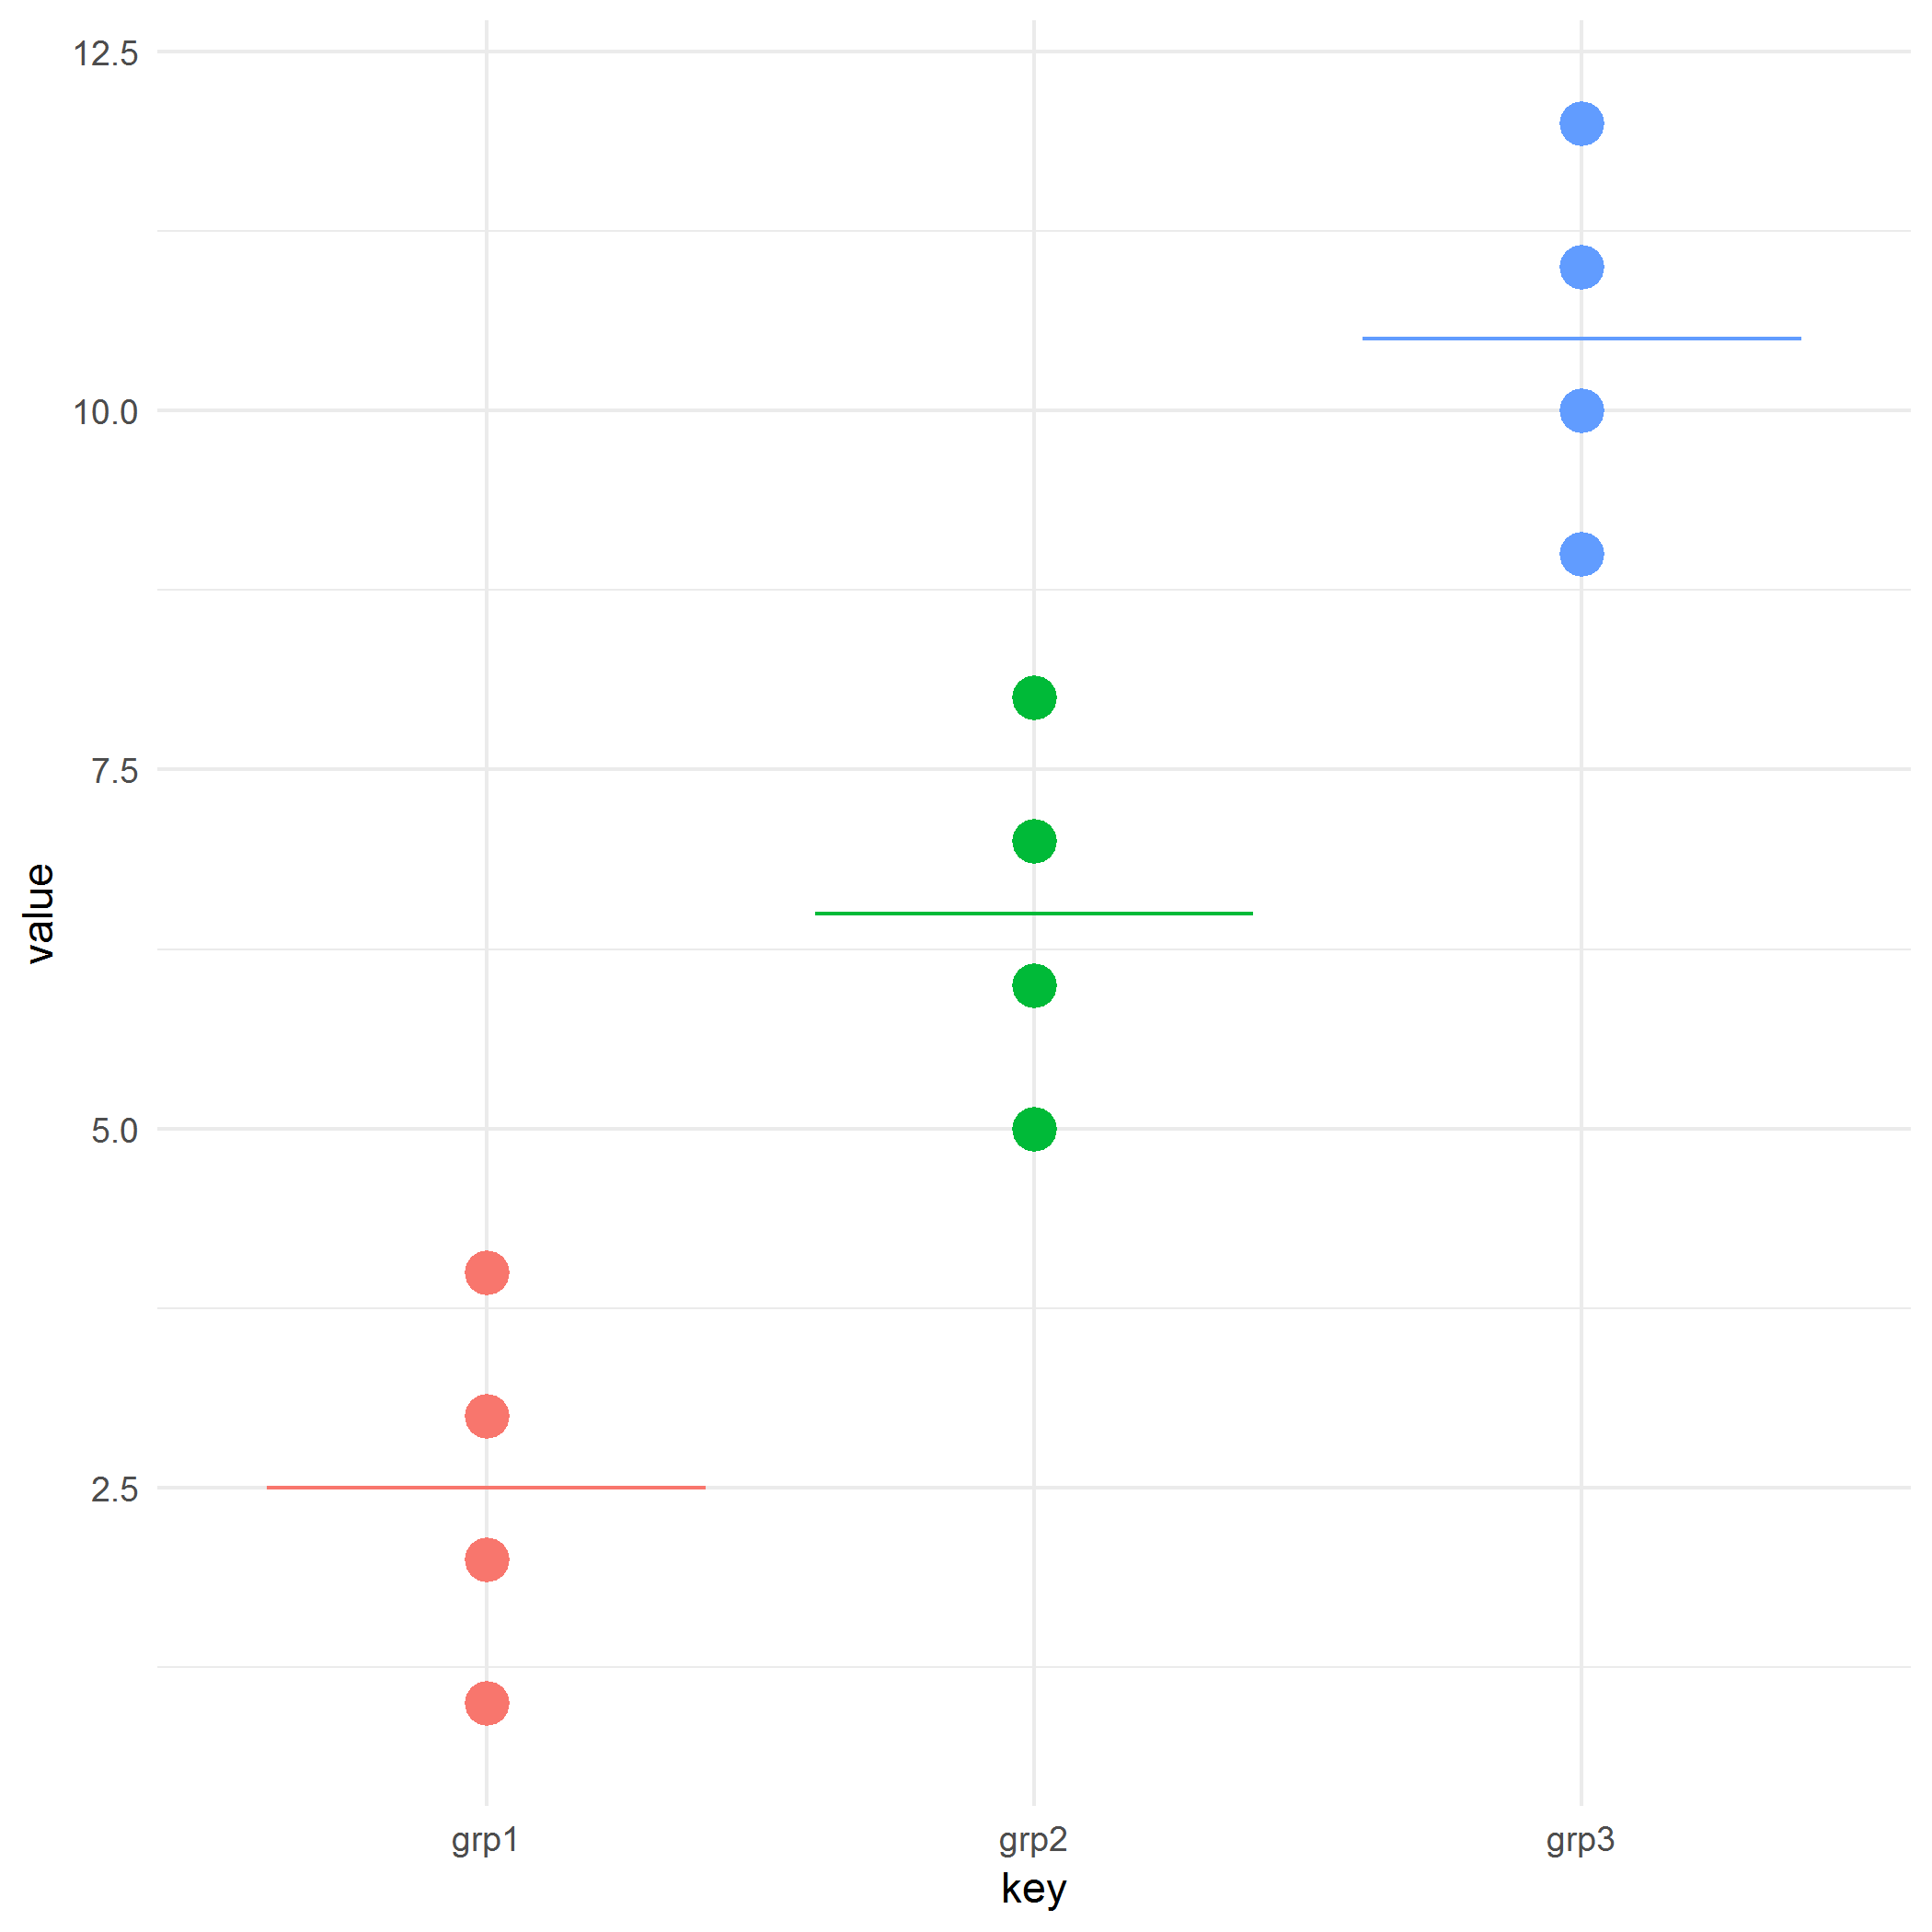
\includegraphics{HW4-key_files/figure-latex/unnamed-chunk-7-1.pdf}

\begin{Shaded}
\begin{Highlighting}[]
\KeywordTok{group_by}\NormalTok{(cuckoos,Bird) }\OperatorTok
\StringTok{  }\KeywordTok{summarise}\NormalTok{(}
    \DataTypeTok{count =} \KeywordTok{n}\NormalTok{(),}
    \DataTypeTok{mean =} \KeywordTok{mean}\NormalTok{(Eggs, }\DataTypeTok{na.rm =} \OtherTok{TRUE}\NormalTok{),}
    \DataTypeTok{sd =} \KeywordTok{sd}\NormalTok{(Eggs, }\DataTypeTok{na.rm =} \OtherTok{TRUE}\NormalTok{)}
\NormalTok{  )}
\end{Highlighting}
\end{Shaded}

\begin{verbatim}
## # A tibble: 6 x 4
##   Bird         count  mean    sd
##   <fct>        <int> <dbl> <dbl>
## 1 HedgeSparrow    14  23.1 1.07 
## 2 MeadowPipit     44  22.2 0.870
## 3 PiedWagtail     15  22.9 1.07 
## 4 Robin           16  22.6 0.685
## 5 TreePipit       16  23.2 0.935
## 6 Wren            15  21.1 0.744
\end{verbatim}

\begin{enumerate}
\def\labelenumi{\alph{enumi}.}
\setcounter{enumi}{1}
\item
\end{enumerate}

\begin{Shaded}
\begin{Highlighting}[]
\NormalTok{cuckmod <-}\StringTok{ }\KeywordTok{lm}\NormalTok{(Eggs }\OperatorTok{~}\NormalTok{Bird, }\DataTypeTok{data =}\NormalTok{ cuckoos)}
\KeywordTok{anova}\NormalTok{(cuckmod)}
\end{Highlighting}
\end{Shaded}

\begin{verbatim}
## Analysis of Variance Table
## 
## Response: Eggs
##            Df Sum Sq Mean Sq F value    Pr(>F)    
## Bird        5 45.938  9.1876  11.478 5.494e-09 ***
## Residuals 114 91.250  0.8004                      
## ---
## Signif. codes:  0 '***' 0.001 '**' 0.01 '*' 0.05 '.' 0.1 ' ' 1
\end{verbatim}

\begin{Shaded}
\begin{Highlighting}[]
\KeywordTok{summary}\NormalTok{(cuckmod)}
\end{Highlighting}
\end{Shaded}

\begin{verbatim}
## 
## Call:
## lm(formula = Eggs ~ Bird, data = cuckoos)
## 
## Residuals:
##    Min     1Q Median     3Q    Max 
##   -2.6   -0.4    0.0    0.6    2.0 
## 
## Coefficients:
##                 Estimate Std. Error t value Pr(>|t|)    
## (Intercept)     23.12143    0.23911  96.697  < 2e-16 ***
## BirdMeadowPipit -0.87143    0.27453  -3.174  0.00193 ** 
## BirdPiedWagtail -0.21810    0.33247  -0.656  0.51316    
## BirdRobin       -0.54643    0.32742  -1.669  0.09788 .  
## BirdTreePipit    0.05357    0.32742   0.164  0.87032    
## BirdWren        -1.99143    0.33247  -5.990  2.5e-08 ***
## ---
## Signif. codes:  0 '***' 0.001 '**' 0.01 '*' 0.05 '.' 0.1 ' ' 1
## 
## Residual standard error: 0.8947 on 114 degrees of freedom
## Multiple R-squared:  0.3349, Adjusted R-squared:  0.3057 
## F-statistic: 11.48 on 5 and 114 DF,  p-value: 5.494e-09
\end{verbatim}

\begin{Shaded}
\begin{Highlighting}[]
\KeywordTok{confint}\NormalTok{(cuckmod)}
\end{Highlighting}
\end{Shaded}

\begin{verbatim}
##                      2.5 %     97.5 %
## (Intercept)     22.6477513 23.5951059
## BirdMeadowPipit -1.4152674 -0.3275897
## BirdPiedWagtail -0.8767168  0.4405263
## BirdRobin       -1.1950379  0.1021808
## BirdTreePipit   -0.5950379  0.7021808
## BirdWren        -2.6500501 -1.3328070
\end{verbatim}

\begin{Shaded}
\begin{Highlighting}[]
\NormalTok{cuckmod1 =}\StringTok{ }\KeywordTok{data.frame}\NormalTok{(}\DataTypeTok{Fitted =} \KeywordTok{fitted}\NormalTok{(cuckmod),}
  \DataTypeTok{Residuals =} \KeywordTok{resid}\NormalTok{(cuckmod), }\DataTypeTok{Birds =}\NormalTok{ cuckoos}\OperatorTok{$}\NormalTok{Bird)}

\KeywordTok{ggplot}\NormalTok{(cuckmod1, }\KeywordTok{aes}\NormalTok{(Fitted, Residuals, }\DataTypeTok{colour =}\NormalTok{ Birds)) }\OperatorTok{+}\StringTok{ }\KeywordTok{geom_point}\NormalTok{()}
\end{Highlighting}
\end{Shaded}

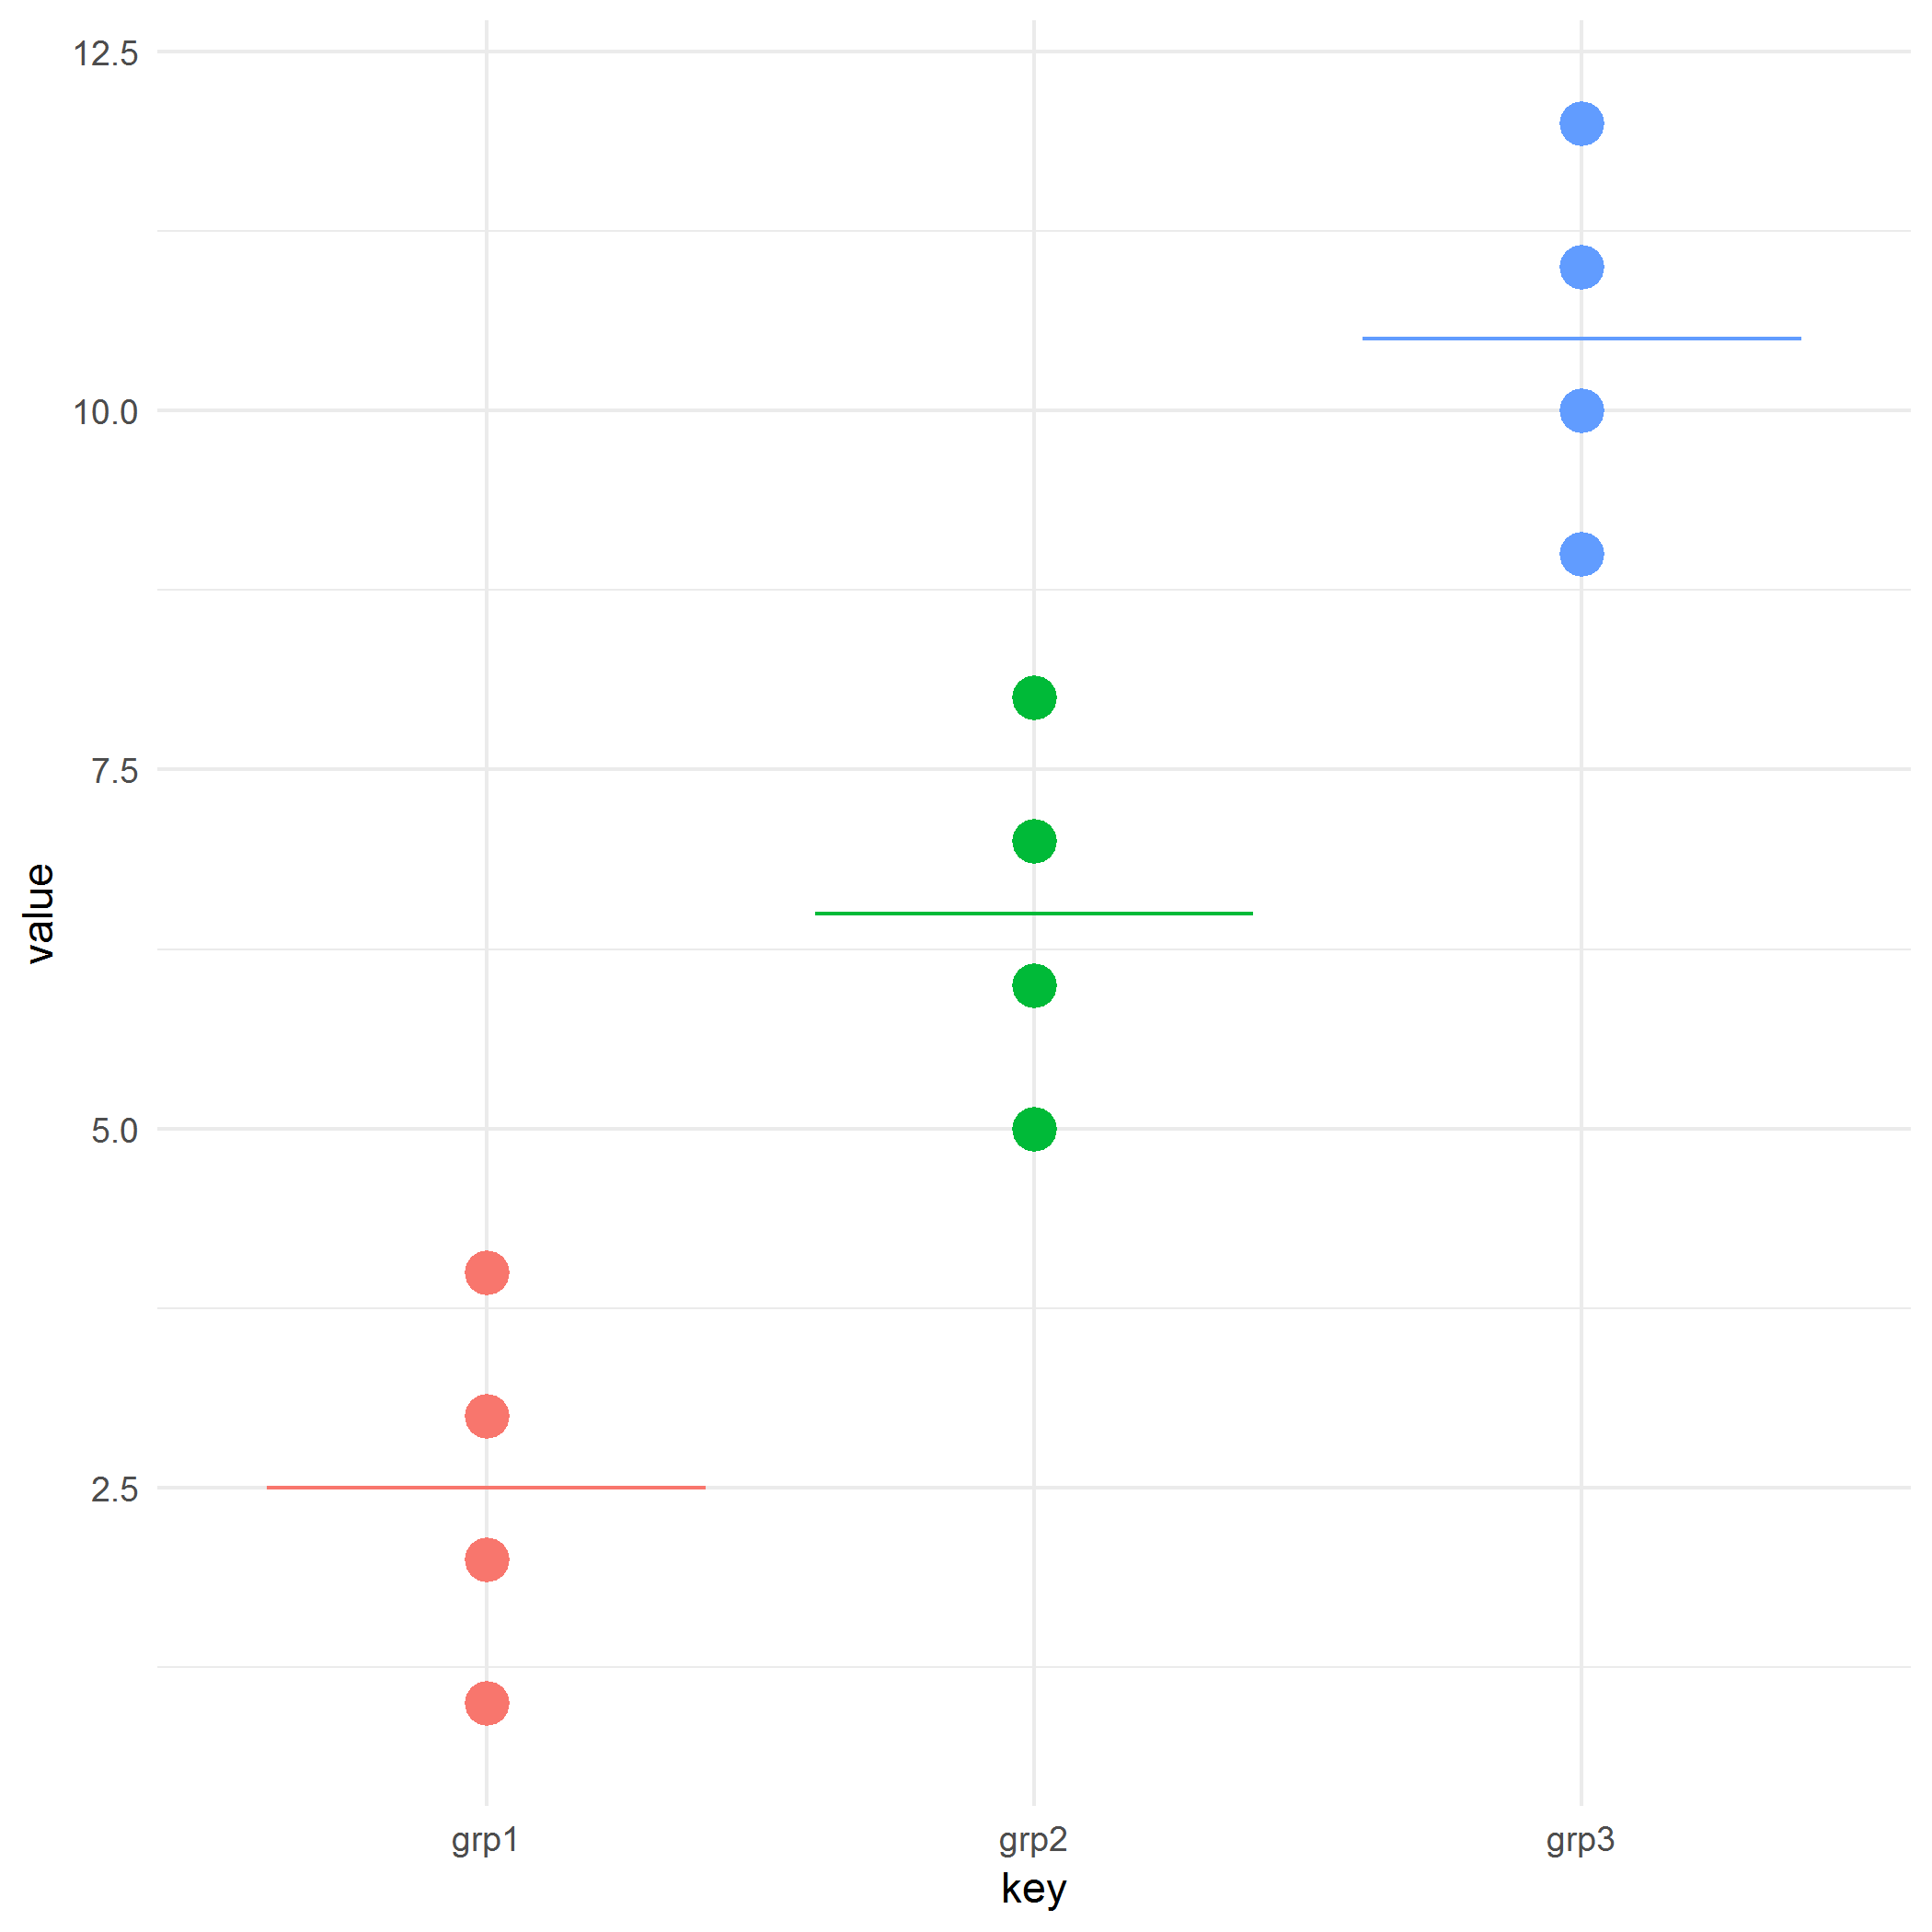
\includegraphics{HW4-key_files/figure-latex/unnamed-chunk-9-1.pdf} c.

\begin{Shaded}
\begin{Highlighting}[]
\NormalTok{aov.fit1 <-}\StringTok{ }\KeywordTok{aov}\NormalTok{(Eggs }\OperatorTok{~}\StringTok{ }\NormalTok{Bird, }\DataTypeTok{data=}\NormalTok{cuckoos)}
\NormalTok{posthoc <-}\StringTok{ }\KeywordTok{TukeyHSD}\NormalTok{(}\DataTypeTok{x=}\NormalTok{aov.fit1, }\DataTypeTok{conf.level=}\FloatTok{0.95}\NormalTok{)}
\NormalTok{posthoc}
\end{Highlighting}
\end{Shaded}

\begin{verbatim}
##   Tukey multiple comparisons of means
##     95% family-wise confidence level
## 
## Fit: aov(formula = Eggs ~ Bird, data = cuckoos)
## 
## $Bird
##                                 diff        lwr         upr     p adj
## MeadowPipit-HedgeSparrow -0.87142857 -1.6672254 -0.07563177 0.0231538
## PiedWagtail-HedgeSparrow -0.21809524 -1.1818530  0.74566255 0.9862488
## Robin-HedgeSparrow       -0.54642857 -1.4955355  0.40267841 0.5550394
## TreePipit-HedgeSparrow    0.05357143 -0.8955355  1.00267841 0.9999833
## Wren-HedgeSparrow        -1.99142857 -2.9551864 -1.02767078 0.0000004
## PiedWagtail-MeadowPipit   0.65333333 -0.1220788  1.42874546 0.1506847
## Robin-MeadowPipit         0.32500000 -0.4321254  1.08212545 0.8140113
## TreePipit-MeadowPipit     0.92500000  0.1678746  1.68212545 0.0074440
## Wren-MeadowPipit         -1.12000000 -1.8954121 -0.34458788 0.0007787
## Robin-PiedWagtail        -0.32833333 -1.2604146  0.60374792 0.9099884
## TreePipit-PiedWagtail     0.27166667 -0.6604146  1.20374792 0.9583313
## Wren-PiedWagtail         -1.77333333 -2.7203288 -0.82633783 0.0000048
## TreePipit-Robin           0.60000000 -0.3169245  1.51692445 0.4094264
## Wren-Robin               -1.44500000 -2.3770813 -0.51291874 0.0002402
## Wren-TreePipit           -2.04500000 -2.9770813 -1.11291874 0.0000001
\end{verbatim}

\begin{Shaded}
\begin{Highlighting}[]
\KeywordTok{plot}\NormalTok{(posthoc)}
\end{Highlighting}
\end{Shaded}

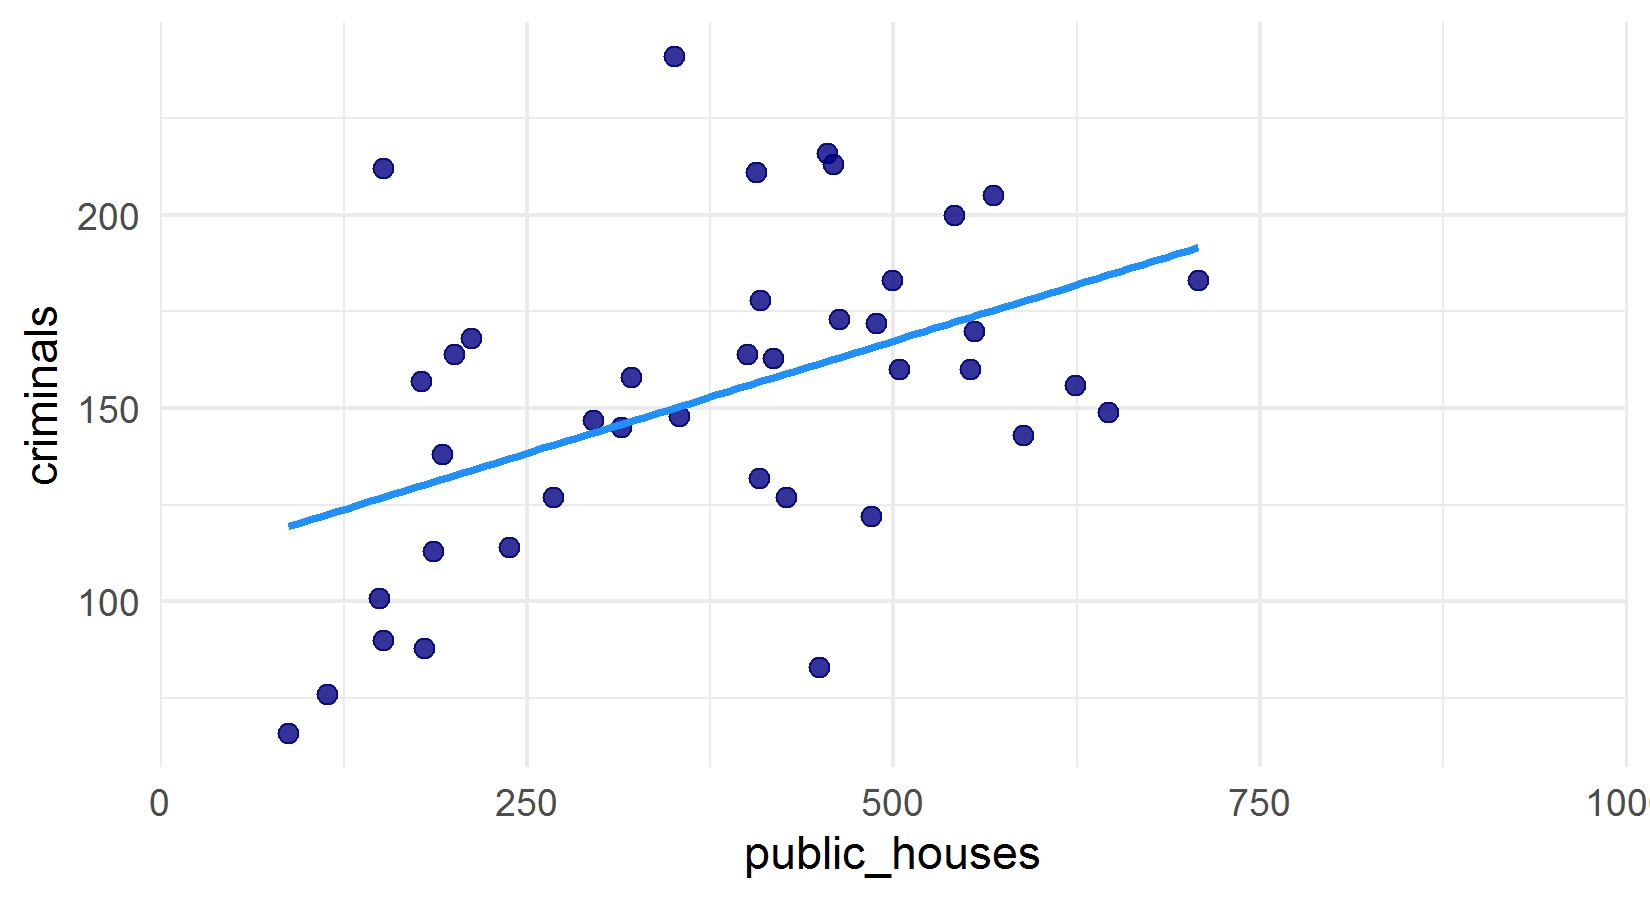
\includegraphics{HW4-key_files/figure-latex/unnamed-chunk-11-1.pdf}

Post-hoc analysis provides insight into any differences between the
groups that may drive the significant omnibus F-statistic found in b.

Looking at the pairwise differences, we see that the below pairs are
significantly different using an un-adjusted p-value of 0.05.

MeadowPipit-HedgeSparrow Wren-HedgeSparrow TreePipit-MeadowPipit
Wren-MeadowPipit Wren-PiedWagtail Wren-Robin Wren-TreePipit

\begin{enumerate}
\def\labelenumi{\alph{enumi}.}
\setcounter{enumi}{3}
\item
\end{enumerate}

\begin{Shaded}
\begin{Highlighting}[]
\NormalTok{posthoc <-}\StringTok{ }\KeywordTok{TukeyHSD}\NormalTok{(}\DataTypeTok{x=}\NormalTok{aov.fit1, }\DataTypeTok{conf.level=}\FloatTok{0.95}\NormalTok{)}
\NormalTok{old <-}\StringTok{ }\KeywordTok{round}\NormalTok{(posthoc}\OperatorTok{$}\NormalTok{Bird[,}\DecValTok{4}\NormalTok{],}\DecValTok{5}\NormalTok{)}
\NormalTok{(adjusted <-}\StringTok{ }\KeywordTok{round}\NormalTok{(}\KeywordTok{p.adjust}\NormalTok{(posthoc}\OperatorTok{$}\NormalTok{Bird[,}\DecValTok{4}\NormalTok{]),}\DecValTok{5}\NormalTok{))}
\end{Highlighting}
\end{Shaded}

\begin{verbatim}
## MeadowPipit-HedgeSparrow PiedWagtail-HedgeSparrow       Robin-HedgeSparrow 
##                  0.20838                  1.00000                  1.00000 
##   TreePipit-HedgeSparrow        Wren-HedgeSparrow  PiedWagtail-MeadowPipit 
##                  1.00000                  0.00001                  1.00000 
##        Robin-MeadowPipit    TreePipit-MeadowPipit         Wren-MeadowPipit 
##                  1.00000                  0.07444                  0.00857 
##        Robin-PiedWagtail    TreePipit-PiedWagtail         Wren-PiedWagtail 
##                  1.00000                  1.00000                  0.00006 
##          TreePipit-Robin               Wren-Robin           Wren-TreePipit 
##                  1.00000                  0.00288                  0.00000
\end{verbatim}

Using a Bonferroni adjusted p-value, we now find only 5 pairs that are
significantly different - those involving Wrens.

Calculation of Familywise Error Rate:

\begin{itemize}
\tightlist
\item
  alpha = 0.05
\item
  c = number of comparisons
\item
  FamilyWiseError = 1 - (1 - aplha)\^{}c
\item
  FamilyWiseError = 1 - (1 - 0.05)\^{}15
\item
  FamilyWiseError = 0.5367
\end{itemize}

Probability of Type I error is over 53\% given 15 comparisons.


\end{document}
